\documentclass{koala-en}
\usepackage[english]{babel}
\usepackage{lastpage}
\usepackage{pdfpages}
\renewcommand{\arraystretch}{1.5} %% Aeration des tableaux
\hyphenpenalty 10000
\usepackage{fancyhdr}
\usepackage{fmtcount}
\pagestyle{fancyplain}
\fancyhf{}
\renewcommand{\chaptermark}[1]{\markboth{#1}{}}
\renewcommand{\sectionmark}[1]{\markright{#1}}
\renewcommand{\headrulewidth}{0.8pt}
\renewcommand{\footrulewidth}{0.8pt}
\fancyhead[R]{\nouppercase{\leftmark}}
\lfoot{Camille Gardet - Internship report - August 2014}
\rfoot{\thepage/\pageref{LastPage}}
\setcounter{secnumdepth}{5}
\setcounter{tocdepth}{5}
\newcommand*{\glossaryname}{Dictionary}
\usepackage{glossaries}
\newcommand{\dictentry}[2]{%
  \newglossaryentry{#1}{name=#1,description={#2}}%
  \glslink{#1}{#1*}%
}
\makeglossaries

%%%%%%%%%%%%%%%%%%%%%%%%%%%%%%%%%%%%%%%%%%%%%%%%

\begin{document}

\title{Internship report}
\subtitle{CS - from  May, \ordinalnum{5} to October, \ordinalnum{7}}

\member{Camille Gardet - }{camille.gardet@epitech.eu}

\summary
{
  This document contains three distinct sections, written in english, intended for three different kind of person :
  \begin{itemize}
     \item A part for a newcomer in the company will resume / continue / maintain the project in which I was involved.
     \item A part to convince my internship supervisor to fit into the team of a new project that I am particularly interested in.
     \item A part to convince a high supervisor (non-technical) to entrust you with the full responsibility for a project, from start to finish, with customer contacts.
  \end{itemize}
  Word with a star in its right upper corner is defined in the glossary at the end of this document. It's clickable (only for numeric version, should I precise this ?).
}

\maketitle

\newpage
\thispagestyle{empty}

\tableofcontents

\thispagestyle{fancy}
\newpage

\part{Documentation for a newcomer}
\chapter{Company presentation}
\section{Sector}
CS is an international company specialized in critical systems of the defense market, security, space, aeronautics and energy.

\begin{figure}[!ht]
  \center
  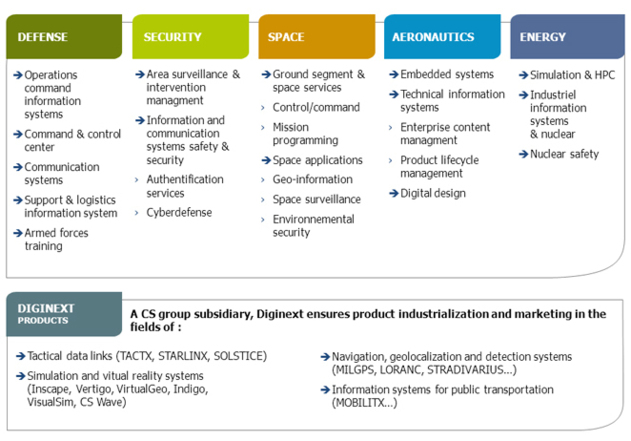
\includegraphics{market.jpg}
  \caption{Critical sectors}
\end{figure}

CS is now a leader in the field of air traffic control. Diginext, a subsidiary of the company, is a leader in \emph{\dictentry{Link 16}{A military tactical data exchange network used by US and NATO. Its specification is part of the family of Tactical Data Links}} and military data links.

\section{Company}
Located in France, Germany, Croatia, Romania, United-Kingdom, Chile, Canada, Emirates, US, Puerto Rico, CS acts all around the world.

\begin{figure}[!ht]
  \center
  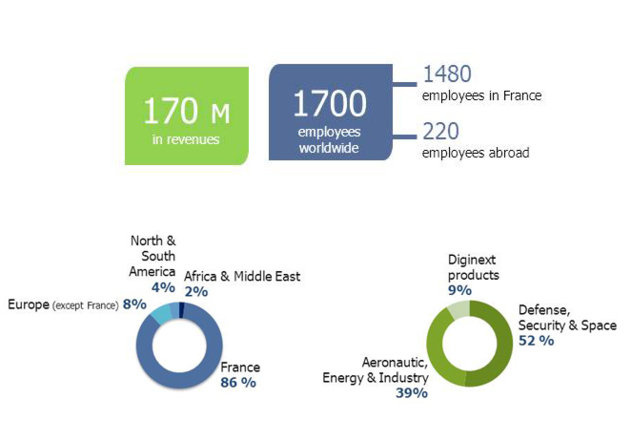
\includegraphics{revenue.jpg}
  \caption{International partners and turnover allocation}
\end{figure}

The company is in partnership with top-notch industrial and commercial company like EADS and Cegelec for air operations, Intel and Wolfram for high performance consulting, Sopra for logistics information systems.

\thispagestyle{fancy}
\newpage

\section{Business unit}

\begin{figure}[!ht]
  \center
  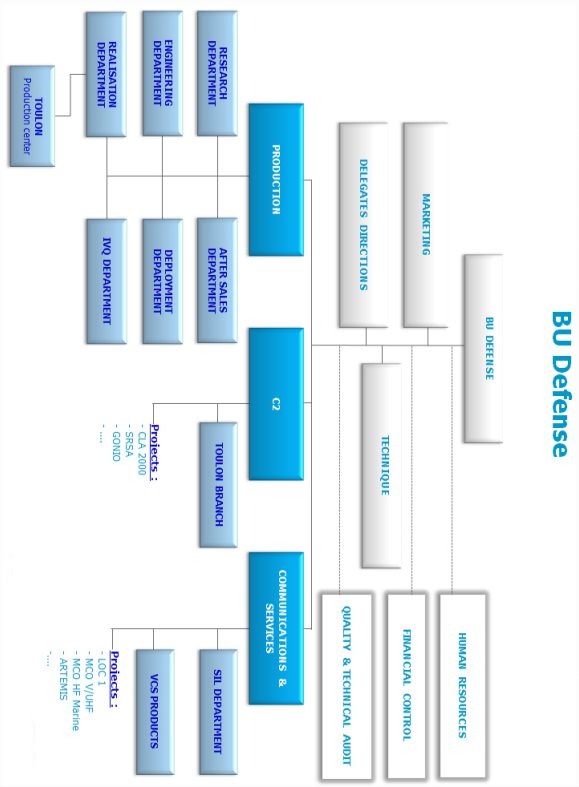
\includegraphics[width=15cm]{ochart.png}
  \caption{Organization chart of the Defense Business Unit}
\end{figure}

The mission of the Defense unit is to implement solutions that meet the internal and external security needs, design and integrate command centers to collect, share and view in real time all the information needed for planning and driving joint army operations.

\section{Contextualization}
CS has had the dual experience, on the one hand of developing security components and solutions, and on the other hand, of managing several e-administration and e-transaction projects. Moreover, backed by its expertise in cryptography and public-key infrastructures, CS offers a complete range of security applications: encryption and implementation in networking equipment, identification and validation, non-reversible transactions, data and interchange confidentiality, secured application flows, and rights management and attribution.
\newline
\newline
In January 2012, CS acquires \emph{Prelude-IDS}, an open-source \dictentry{SIEM}{Security Information \& Event Management - Provide real-time analysis of security alerts generated by network hardware and applications}, and puts a lot of effort to rebuild it, and puts it back online.

\thispagestyle{fancy}
\newpage

\chapter{Prelude}
\section{Definition - What is Prelude ?}

\begin{figure}[!ht]
  \center
  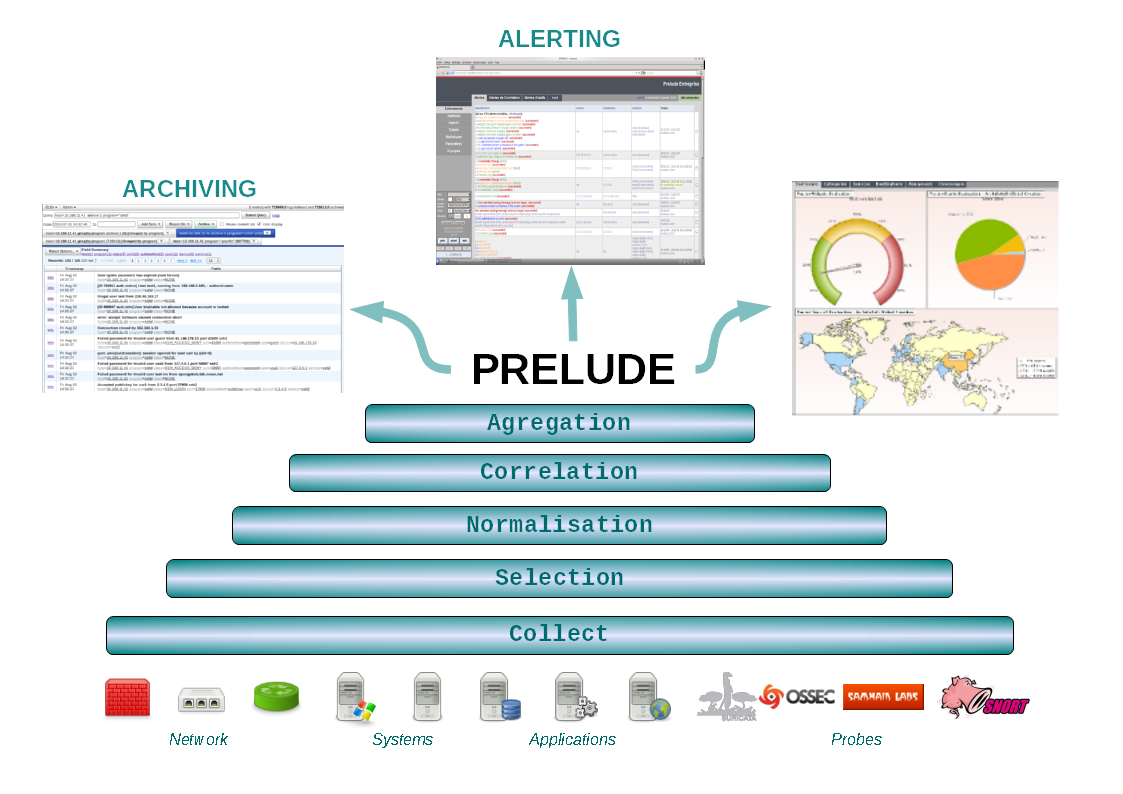
\includegraphics[width=15cm]{archi-simple.png}
  \caption{General overview}
\end{figure}

Prelude is a universal \emph{Security Information \& Event Management} (\dictentry{SIEM}{Security Information \& Event Management - Provide real-time analysis of security alerts generated by network hardware and applications}) system. Prelude collects, normalizes, sorts, aggregates, correlates and reports all security-related events independently of the product brand or license giving rise to such events.
\newline
\newline
As well as being capable of recovering any type of log (system logs, syslog, flat files, etc.), Prelude benefits from a native support with a number of systems dedicated to enriching information even further (snort, samhain, ossec, auditd, etc.).
\newline
\newline
Security events are normalized thanks to a single format, called the \emph{Intrusion Detection Message Exchange Format} (\dictentry{IDMEF}{Intrusion Detection Message Exchange Format - define data formats and exchange procedures for sharing information of interest to intrusion detection and response systems and to the management systems that may need to interact with them}), which is an international standard created upon the initiative of \dictentry{IETF}{Internet Engineering Task Force - develops and promotes voluntary Internet standards} along with the participation of Prelude teams to enable interacting with the various security tools currently available on the market.


\section{How does it work ?}

\begin{figure}[!ht]
  \center
  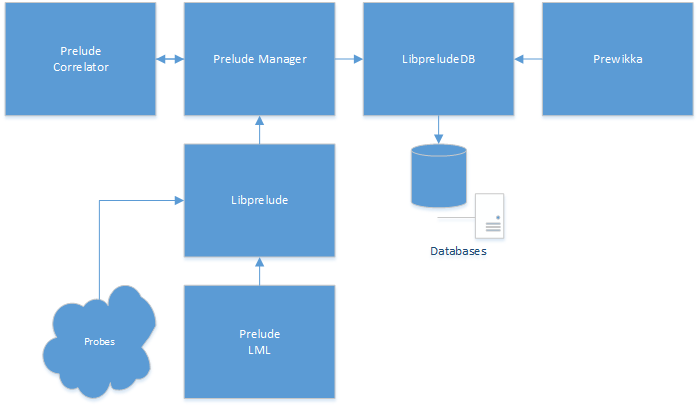
\includegraphics[width=15cm]{prelude.png}
  \caption{Communication between elements}
\end{figure}

\emph{Prelude LML} monitors system activites and read logfile generated by any kind of probes and create \dictentry{IDMEF}{Intrusion Detection Message Exchange Format - define data formats and exchange procedures for sharing information of interest to intrusion detection and response systems and to the management systems that may need to interact with them} alerts with \emph{Libprelude}.
\newline
\newline
\emph{Libprelude} is a library used to make \dictentry{IDMEF}{Intrusion Detection Message Exchange Format - define data formats and exchange procedures for sharing information of interest to intrusion detection and response systems and to the management systems that may need to interact with them} alerts and agent, to connect to a data bus (here, \emph{Prelude Manager}).
\newline
\newline
\emph{Prelude Manager} is a server with secured connections, which receives alerts and write it on any kind of support, like databases or files.
\newline
\newline
\emph{LibpreludeDB} is an abstraction to interface the manager with any kind of databases (pgsql, mysql, sqlite).
\newline
\newline
\emph{Prelude Correlator} is a correlation factory, which is allowed to create new alert based on multiple alert.
\newline
\newline
\emph{Prewikka} is the GUI of Prelude. Web-based, it shows alerts, correlated alerts, probes states, statistics about systems, alerts, and so on.

\chapter{Latest developments - Documentations}
Prelude is an old and open-source based project without any user or developer documentations.
\newline
\newline
A part of the mission involve to write these documentations, helped with the reference document of CS :
\begin{itemize}
  \item System/Subsystem Specification (SSS) - The requirements to be met by the system,
  \item System/Subsystem Design Description (SSDD) - The design of the system
\end{itemize}

Each module of Prelude must be covered. \emph{Libprelude} documentation is already written and will be used as example in this document. Guidelines to write these documents are provided below.

\thispagestyle{fancy}
\newpage

\section{System/Subsystem Specification (SSS)}
\subsection{Needs}
Understanding the needs is the first thing to know and answer questions like \emph{Why do I need this ?} or \emph{How can I fulfill this requirements ?}. The requirements are submited by the client, most of time, but also by CS, to match a local standard.

\subsection{Technical requirements}
\emph{How things should work ?}
\newline
While being general, each features of a module are formated as a requirement, describing its operating.
A small flow-chart to illustrate this is strongly recommended.

\begin{figure}[!ht]
  \center
  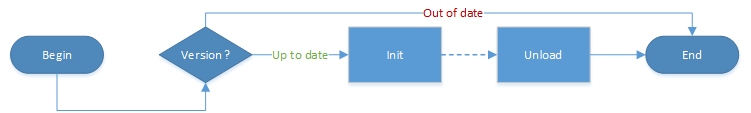
\includegraphics[width=15cm]{sss.png}
  \caption{Init Libprelude - How should it proceeds}
\end{figure}

Followed by :
\begin{lstlisting}
  LIB_USE_VERSION : Check library version
  How : Use a function to return the version
  Why : The version can be checked before the initialisation

  ...
\end{lstlisting}
Same for the init and unload part.

\subsection{External interface requirements}
\emph{What will provide external connection ?}
\newline
Not only network of course. Everything that will communicate/use/connect to the module is an external interface.
It can be other module of the project, external library, \dictentry{API}{Application Programming Interface - specifies how some software components should interact with each other}, language binding, etc.

\subsection{Internal interface requirements}
\emph{What use my module to run properly ?}
\newline
If the module use a configuration file, or data in a specified standard format, it should be listed as an internal interface. For example, the IDMEF format is specified in a \dictentry{RFC}{Request For Comments - the principal technical development and standards-setting bodies for the Internet}.

\subsection{Environment requirements}
Everything environment related, like \emph{Should my library be crossplatform ?} or \emph{What happens when my system reboot ?}.

\subsection{Definition and conception constraints}
Languages or tools that \textbf{must} be used to implement the module. \emph{Libprelude} must be written in C for example.

\thispagestyle{fancy}
\newpage

\section{System/Subsystem Design Description (SSDD)}
\subsection{Design principle}


\subsection{System structure}
tba

\thispagestyle{fancy}
\newpage

\chapter{Latest developments - Coding}
\section{CS standard}
To develop features on Prelude, it's recommended to use :
\begin{itemize}
  \item CentOS 6 virtual machine,
  \item Python 2,
  \item C, standard C89,
  \item Redmine, for project management and bug-tracking tool,
  \item Latest version of Prelude, found on \url{http://www.prelude-ids.org}
\end{itemize}

\section{A new probe, Motion}
Using a webcam, the probe should be able to raise alert when it detects movement. \emph{How ?}
\subsection{Motion ?}
Motion is a small tool to monitor video streams, coming from one or many video device and is able to detect movement.
\newline
\newline
The tool is written in C for linux based OS.
\newline
\newline
Since its version 3.1.12, the tool is maintained by Kenneth Lavrsen and a small community.
\newline
Homepage : \url{http://www.lavrsen.dk/foswiki/bin/view/Motion/WebHome}

\subsection{Implementation}
Using libprelude, where to plug it
\subsection{Results}
screenshots

\section{Enhance statistics in Prewikka}
\subsection{One library, to rule them all}
d3js
\subsection{Implementation}
template, views, filter, list of graphics, only js
first -> csv
final -> libpreludeDB
\subsection{Results}
screenshots!

\section{Make GeoIP customisable}
\subsection{GeoIP ?}
what is geoip
\subsection{Implementation}
template, view, csv/dat, python part
\subsection{Results}
screenshots!!

\chapter{Final word}

\thispagestyle{fancy}
\newpage

%% Lexicon

\printglossary[style=altlisthypergroup]
\addcontentsline{toc}{chapter}{Glossary}

\thispagestyle{fancy}
\end{document}
